\section{Methodology}
\label{sec:methodology}
In this section, we cover the development of the three KGs, (\textbf{$\mathbb{G}_1$} (T2DM-focused), \textbf{$\mathbb{G}_2$} (AD-focused), and \textbf{$\mathbb{G}_3$} (combined AD+T2DM)), the creation of the probes and the experimentation of the seven LLMs with different combinations of the knowledge graphs, shown in Figure \ref{fig:framework}. 

\subsection{Abstract Selection  and Filtration}

\begin{ashbox}
\textbf{Search queries used to build the KG sets} 

\vspace{0.4em}
\noindent\textbf{$Q_{T2DM}$ (T2DM-only).}\\
\texttt{(T2DM OR "Type 2 Diabetes" OR "Type II Diabetes" OR "Type-2 Diabetes" OR "Diabetes Mellitus, Type 2" OR NIDDM OR "non insulin dependent diabetes" OR "non-insulin-dependent diabetes" OR "adult-onset diabetes" OR (diabet* AND ("type 2" OR T2DM)))}

\vspace{0.4em}
\noindent\textbf{$Q_{AD}$ (AD-only).}\\
\texttt{(AD OR "Alzheimer's disease" OR "Alzheimer disease" OR "Alzheimers disease" OR Alzheimers OR Alzheime* OR Alzhiemer* OR "dementia of the Alzheimer type" OR DAT OR LOAD OR "late-onset Alzheimer*")}

\vspace{0.4em}
\noindent\textbf{$Q_{T2DM + AD}$ (AD \& T2DM together).}\\
\texttt{((AD OR "Alzheimer* disease" OR Alzheime* OR Alzhiemer* OR DAT OR LOAD) AND (T2DM OR "Type 2 Diabetes" OR "Type II Diabetes" OR "Diabetes Mellitus, Type 2" OR NIDDM))}

\end{ashbox}

After applying the $Q_{T2DM}$/$Q_{AD}$/$Q_{AD + T2DM}$ search strings, we created a simple, reproducible filter to rank abstracts and kept the most relevant \emph{per group}. The aim is to bias toward causal and mechanistic content while still covering phenotypes and biomarkers that matter for AD, T2DM, and their intersection. We remove short-worded abstracts (less than 180 words) to avoid editorials or thin notes:
\[
\text{keep}(i)\;=\;\mathbb{1}\big[\mathrm{words}(\texttt{Abstract}_i)\ge 180\big].
\]
We then join title and abstract into one text string $x_i$, and build a TF--IDF matrix on unigrams and bigrams (English stopwords, \texttt{min\_df}=2):
\[
X \in \mathbb{R}^{n \times V},\qquad X_i=\mathrm{tfidf}(x_i),\quad i=1\ldots n.
\]
We create three query vectors by TF--IDF, transforming the curated term lists:
\[
q_{\mathrm{caus}},\ q_{\mathrm{pheno}},\ q_{\mathrm{biom}} \;\in\; \mathbb{R}^V,
\]
representing  \texttt{CAUSALITY\_TERMS}, \texttt{PHENOTYPE\_TERMS}, and \texttt{BIOMARKER\_TERMS} respectively. For each abstract, we compute three cosine similarities:
\[
s^{(\mathrm{caus})}_i=\cos(X_i,q_{\mathrm{caus}}),\quad
s^{(\mathrm{pheno})}_i=\cos(X_i,q_{\mathrm{pheno}}),\quad \]
\[
s^{(\mathrm{biom})}_i=\cos(X_i,q_{\mathrm{biom}}).
\]

We reward abstracts that explicitly name crucial elements (e.g., “Mendelian randomization,” “longitudinal,” “p-tau-217,” “APOE4,” “insulin resistance phenotype,” “HbA1c”).
\[
k^{(\mathrm{caus})}_i,\ k^{(\mathrm{pheno})}_i,\ k^{(\mathrm{biom})}_i \in \mathbb{N},\qquad
k^{(\mathrm{tot})}_i = k^{(\mathrm{caus})}_i + k^{(\mathrm{pheno})}_i + k^{(\mathrm{biom})}_i.
\]


\paragraph*{Per-feature normalization.}
Each signal is min--max normalized to $[0,1]$ to keep ranges comparable:
\[
\tilde{s}^{(\cdot)}_i=\frac{s^{(\cdot)}_i-\min s^{(\cdot)}}{\max s^{(\cdot)}-\min s^{(\cdot)}},\quad
\tilde{k}_i=\frac{k^{(\mathrm{tot})}_i-\min k^{(\mathrm{tot})}}{\max k^{(\mathrm{tot})}-\min k^{(\mathrm{tot})}}.
\]
We then produce a single value that we use \emph{only to rank} abstracts:
\[
R_i \;=\; w_{\mathrm{caus}}\tilde{s}^{(\mathrm{caus})}_i
\;+\; w_{\mathrm{pheno}}\tilde{s}^{(\mathrm{pheno})}_i
\;+\; w_{\mathrm{biom}}\tilde{s}^{(\mathrm{biom})}_i \]
\[
\;+\; w_{\mathrm{kw}}\tilde{k}_i.\]

The final KGs were created from the top 1000 selected abstracts. 

\begin{figure*}[htbp]
 \centering
 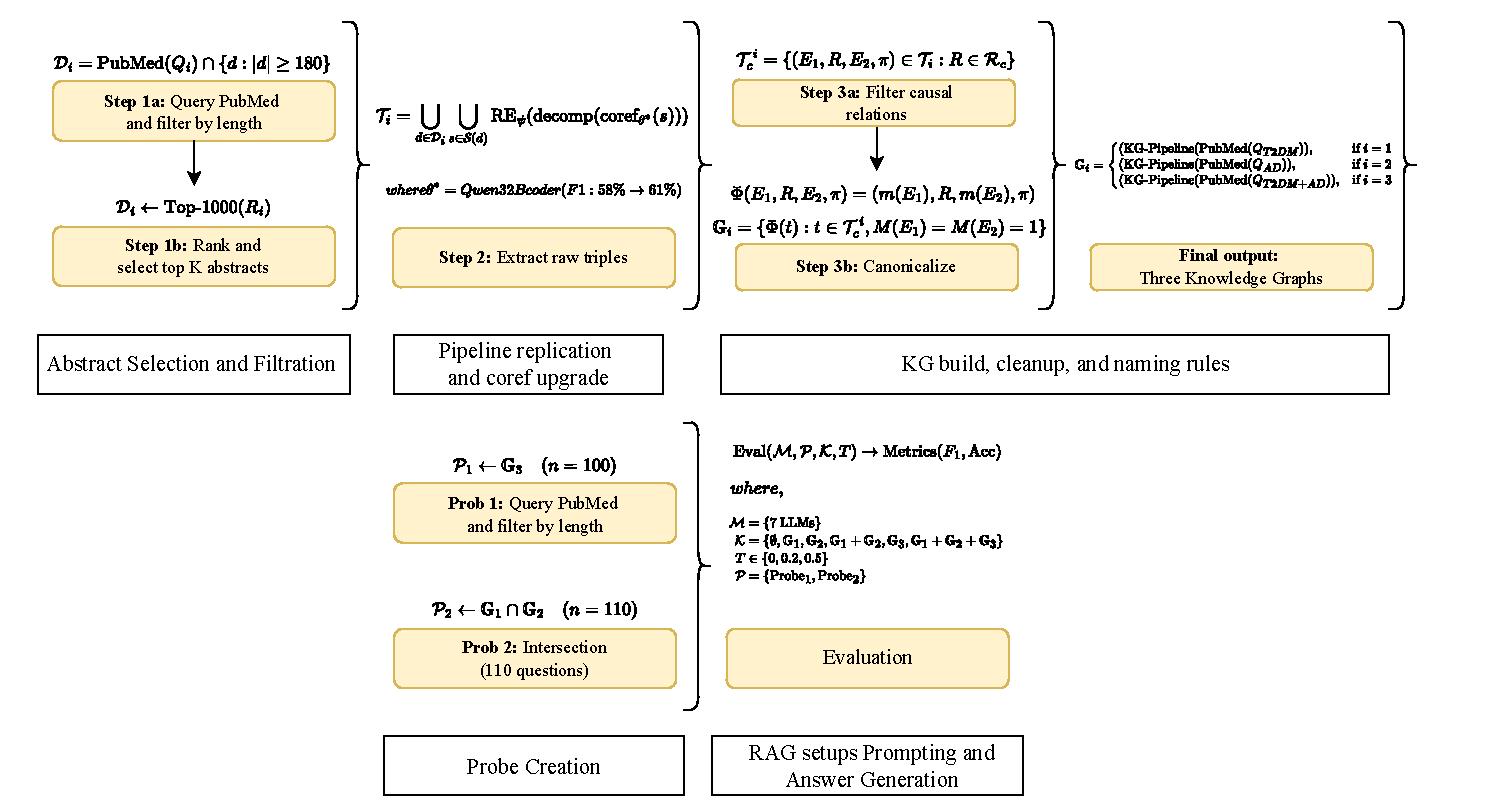
\includegraphics[width=1\textwidth]{images/Domain-Specific KG.drawio_v7.0.pdf}
 \caption{Overview of the methodology for constructing domain-specific knowledge graphs and evaluating their impact on RAG-enhanced healthcare LLMs. The pipeline includes abstract selection, knowledge graph construction, probe generation, and systematic evaluation across multiple models and retrieval configurations. Detailed explanation is provided in Section \ref{sec:methodology}.}
\label{fig:framework}
\vspace{-3mm}
\end{figure*}


\subsection{Pipeline replication and coref upgrade}
We start from the selected abstracts $\mathcal{D}=\{d_1,\ldots,d_N\}$ and treat each abstract as a set of sentences $\mathcal{S}(d)=\{s_1,\ldots,s_{|d|}\}$. The extraction loop in \textsc{CoDe-KG} is
\begin{equation}
\label{eq:pipeline}
\mathcal{T} \;=\; \bigcup_{d\in\mathcal{D}} \;\; \bigcup_{s\in \mathcal{S}(d)} \; \mathrm{RE}_\psi\!\left(\mathrm{decomp}\!\left(\mathrm{coref}_\theta(s)\right)\right),
\end{equation}
where  $s$ (\textit{coref}) $\rightarrow$ is resolving abstract co-reference, i.e ``T2DM" = ``Type 2 Diabetes Mellitus" = ``t2dm"; then decompose complex sentences into simpler ones (\textit{decomp}), then extract triples $(E_1, R, E_2)$ with a simple source tag $\pi(t)$ that notes (paper id, sentence id, clause id). This tag lets us always point back to the exact sentence that created a triple. We first matched the original authors’ inference setting (temp $=0.7$) and reproduced similar relation extraction behavior. We replaced the coreference backbone with {Qwen~32B coder} and kept all other steps the same.
\[
\mathrm{coref}_{\theta^\star} \text{ reaches } \mathrm{F1}=61\% \text{ vs. } 58\% \text{ before,}
\]
This test was done on the authors dataset. In practice, better coref means fewer broken heads or tails later, so the KG has cleaner nodes and more usable causal links.

\subsection{KG build, cleanup, and naming rules}
Raw extraction gives a multi-set of triples $\mathcal{T}$. For our study, we want edges that point in a clear causal direction, so we kept only a small relation set. 
\[
\mathcal{R}_c=\{\texttt{causes},\ \texttt{because}, ...\}.
\]
Formally,
\begin{equation}
\label{eq:causal-filter}
\mathcal{T}_c \;=\; \{\, (E_1, R, E_2,\pi) \in \mathcal{T} \;:\; r\in \mathcal{R}_c \,\}.
\end{equation}
Next, we remove vague heads/tails. A simple mask $M$ drops items like ``it'', ``this'', or ``this study'':
\[
M(x)=\mathbb{1}\!\left[x \notin \{\texttt{it},\texttt{this},\texttt{this study}\} \right],
\]
\[
\qquad
\mathcal{T}_{c}^{\mathrm{clean}}=\{t\in\mathcal{T}_c: M(E_1)=M(E_2)=1\}.
\]

We manually normalize names so variants collapse to a single label: ``T2DM'' and ``Type~2~Diabetes'' should be treated as one thing. We rewrite each edge by
\[
\Phi:\ (E_1, R, E_2,\pi)\mapsto \big(m(E_1),\,R,\,m(E_2),\,\pi\big),
\]
and obtain the canonical set $\widehat{\mathcal{T}}_c=\{\Phi(t):t\in\mathcal{T}_c^{\mathrm{clean}}\}$.

\subsection{Probe Creation}
We created two types of Probes: the first built on $\mathbb{G}_3$ and the second built on the intersection of $\mathbb{G}_1$ and $\mathbb{G}_2$ $\rightarrow (\mathbb{G}_1 \cap \mathbb{G}_2)$

\subsubsection{Probe 1}
Containing 100 multiple-choice questions, this probe tests the joint AD+T2DM query. The questions are framed to cover single hop, multi-hop and fill in the blank (FITB).  Let $A\in\{0,1\}^{|\widehat{\mathcal{E}}_3|\times|\widehat{\mathcal{E}}_3|}$ be the adjacency over $\mathcal{R}_c$.
\begin{itemize}
  \item \textbf{Single-hop.} Choose $(u,r,v)\!\in\!\widehat{\mathcal{T}}_{c,3}$ and create one correct option and three distractors from $\mathcal{N}^{-}(u)=\{x:A_{x,u}=1\}$ that match type/frequency. This checks one clean link.
  \item \textbf{Multi-hop, pair-selection.} For a target $x$, the set of \emph{direct} causes is $\mathcal{P}_1(x)=\{u:A_{u,x}=1\}$. The correct answer is an unordered pair $\{u,v\}\subseteq\mathcal{P}_1(x)$. Distractors come from $\mathcal{P}_2(x)=\{u:(A^2)_{u,x}=1\}$ or close neighbors that look right but are not immediate parents. This stresses real 2-hop reasoning.
  \item \textbf{FITB.} Mask one canonical token in $(u,r,v)$; only the canonical label passes. This drills precision under synonyms.
\end{itemize}
We ensure synonym control explicitly, as options must be distinct in canonical space ($m(c_i)\neq m(c_j)$), so there are no duplicate answers under different spellings.


\begin{table*}[ht]
\centering
\caption{QA items formatted as fill-in-the-gap, multi-hop, and single-hop examples.}
\scriptsize
\setlength{\tabcolsep}{4pt}
\renewcommand{\arraystretch}{1.15}
\begin{adjustbox}{max width=\linewidth}
\begin{tabularx}{\linewidth}{
  >{\raggedright\arraybackslash}p{.16\linewidth}
  >{\raggedright\arraybackslash}p{.36\linewidth}
  >{\raggedright\arraybackslash}p{.22\linewidth}
  >{\raggedright\arraybackslash}p{.26\linewidth}}
\toprule
\textbf{Question type} & \textbf{Question} & \textbf{Options} & \textbf{Answer choices} \\
\midrule
Fill-in-the-gap &
Type 2 diabetes increases Alzheimer’s risk through \underline{\hspace{1.2cm}} and \underline{\hspace{1.2cm}}. &
\begin{tabular}[t]{@{}l@{}}
1. Neuroinflammation\\
2. Amyloid degradation\\
3. Insulin resistance\\
4. Tau dephosphorylation
\end{tabular} &
\begin{tabular}[t]{@{}l@{}}
A: 1 and 2\\
B: 3 and 4\\
C: 3 and 2\\
D: 2 and 4\\
E: 3 and 1
\end{tabular}
\\
\addlinespace
Multi-hop &
Which two are direct precursors of neuroinflammation escalation? &
\begin{tabular}[t]{@{}l@{}}
1. A$\beta$ oligomers\\
2. Peripheral infection\\
3. Aerobic fitness\\
4. Microglial priming
\end{tabular} &
\begin{tabular}[t]{@{}l@{}}
A: 1 and 2\\
B: 1 and 4\\
C: 2 and 3\\
D: 3 and 4
\end{tabular}
\\
\addlinespace
Single-hop &
Abnormal insulin signaling in the brain primarily results in: &
\begin{tabular}[t]{@{}l@{}}
A: Lower GSK3$\beta$ activity\\
B: Reduced oxidative damage\\
C: Enhanced mitochondrial function\\
D: Higher synaptic resilience\\
E: Reduced A$\beta$ degradation and increased tau phosphorylation
\end{tabular} &
— \\
\bottomrule
\end{tabularx}
\end{adjustbox}
\label{tab:qa_items}
\end{table*}



\subsubsection{Probe 2}
This probe targets $\mathbb{G}_1 \cap \mathbb{G}_2$. We embed the triple with an encoder $s(\cdot)\in\mathbb{R}^d$ and use cosine similarity to screen for intersection candidates $\mathcal{I}$
\begin{equation}
\label{eq:cos-thresh}
\mathcal{I} \;=\; \Big\{ (\tau_1,\tau_2)\in \widehat{\mathcal{T}}_{c,1}\!\times\!\widehat{\mathcal{T}}_{c,2}:\ \mathrm{cos}\!\left(s(\tau_1),s(\tau_2)\right)\ge 0.65 \Big\}.
\end{equation}
Yielding $|\mathcal{I}|=424$. After stop-word removal and de-duplication in canonical space, we keep $|\widehat{\mathcal{I}}|=193$ items. We then form questions from this intersection subgraph:
\begin{itemize}
  \item \textbf{Single-hop, FITB:} Same as Probe~1 but restricted to $\widehat{\mathcal{I}}$.
  \item \textbf{Multi-hop with direction.} If the true edge is $u\!\to\!x$, then the option $x\!\to\!u$ is wrong even though it uses the same names. We present four atomic options (1--4) and ask for the correct pair among A--E (the 2-combinations). Exactly two pairs are correct; both must point into the target.
\end{itemize}
0.65 was chosen as the cosine similarity value because it kept the same causal theme in both diseases (e.g., insulin signaling, inflammation) without having too loose matches.

\subsection{RAG setups Prompting and Answer Generation}
We compare six retrieval setups:
\[
K \in \big\{\varnothing\,,\ \mathbb{G}_1,\ \mathbb{G}_2,\ \mathbb{G}_1\!+\!\mathbb{G}_2,\ \mathbb{G}_3,\ \mathbb{G}_1\!+\!\mathbb{G}_2\!+\!\mathbb{G}_3\big\}.
\]

Where $\varnothing\ \rightarrow \text{(No-RAG)}$. For each value of $K$, we run the same LLM with and without this context. For QA we use $T\in\{0,0.2,0.5\}$; Lower $T$ sticks closer to retrieved facts; higher $T$ can add details but risks drift.
All the prompts were zero-shot instruction based. 
\begin{ashbox}
\ttfamily
You are answering a multiple-choice question.\\
Return ONLY one uppercase letter from this set: \{allowed\_str\}.\\
Do not include explanations or extra text.
\end{ashbox}

Since all questions were multiple-choice, we incorporated common distractors in the options. For questions with multiple answers, we tested the macro and micro F1 in those cases.

